% TRIAD on one real POG_DENSE test query (seed-0 model, query #165): how the hidden item is scored, lane by lane.
% Images: pog/*.png (released POG product images). Build: pdflatex architecture_example.tex
\documentclass[tikz,border=5pt]{standalone}
\usepackage{amsmath,amssymb}
\usepackage{fontawesome5}
\usetikzlibrary{arrows.meta,calc,positioning,backgrounds}
\renewcommand{\familydefault}{\sfdefault}
\definecolor{fzfill}{HTML}{E3EFFA}\definecolor{fzline}{HTML}{3B7FC4}
\definecolor{trfill}{HTML}{FDE6CF}\definecolor{trline}{HTML}{D9730D}
\definecolor{cX}{HTML}{6FA8DC}\definecolor{cH}{HTML}{B4A7D6}
\definecolor{cC}{HTML}{7B4FB8}\definecolor{cL}{HTML}{1C9A8A}\definecolor{cG}{HTML}{3A8F3A}\definecolor{cS}{HTML}{C8372D}
\newcommand{\fire}{{\color{trline}\faFire}}
\newcommand{\snow}{{\color{fzline}\faSnowflake}}
\tikzset{
  arr/.style={-{Stealth[length=2.4mm]},line width=0.9pt,draw=black!60},
  lane/.style={rounded corners=8pt,line width=0},
  colhead/.style={font=\bfseries\normalsize,align=center},
  lanehead/.style={font=\bfseries\large,anchor=west},
  lbl/.style={font=\normalsize,align=center},
  small/.style={font=\small,align=center,text=black!75},
  fz/.style={draw=fzline,fill=fzfill,line width=1pt,rounded corners=3pt,font=\normalsize,align=center,inner sep=4pt},
  tr/.style={draw=trline,fill=trfill,line width=1pt,rounded corners=3pt,font=\normalsize,align=center,inner sep=4pt},
  val/.style={draw=#1,fill=#1!10,line width=1.2pt,rounded corners=4pt,font=\large,align=center,inner sep=5pt,minimum width=3.0cm},
  op/.style={circle,draw=black!70,line width=0.9pt,minimum size=6.5mm,inner sep=0pt,fill=white,font=\normalsize},
  img/.style={draw=black!25,line width=0.5pt,inner sep=0pt},
}
\newcommand{\vrow}[6]{\foreach \i in {1,...,#3}{\draw[black!55,fill=#4,line width=0.4pt] ($(#1,#2)+({(\i-1)*#5},0)$) rectangle ++(#5,#6);}}
\newcommand{\itemimg}[4]{\node[img] (#1) at #3 {\includegraphics[width=#4]{pog/#2.png}};}
\newcommand{\curve}[3]{\draw[trline,line width=1.2pt] ($(#1,#2)+(-0.45,-0.2)$) .. controls ($(#1,#2)+(-0.15,#3)$) and ($(#1,#2)+(0.1,-0.25)$) .. ($(#1,#2)+(0.45,0.22)$);}

\begin{document}
\begin{tikzpicture}[x=1cm,y=1cm]

% ===================================================================== QUERY
\node[font=\bfseries\large,anchor=west] at (0,21.4) {A query and one candidate};
\itemimg{bag}{seed_10091}{(0.9,20.0)}{1.6cm}
\itemimg{ear}{seed_30318}{(2.75,20.0)}{1.6cm}
\draw[black!55,rounded corners=5pt,line width=0.9pt] (-0.05,19.05) rectangle (3.7,21.0);
\node[lbl,anchor=north] at (1.82,18.95) {seeds $S$};
\itemimg{cand}{hidden_16088}{(6.2,20.0)}{1.6cm}
\node[lbl,anchor=north] at (6.2,18.95) {candidate $c$ (the hidden item)};
\node[lbl,anchor=west,align=left,font=\large] at (8.6,20.0) {How likely is $c$ to complete the outfit?\\[3pt]
  TRIAD answers with three terms, \textcolor{cC}{$C$}, \textcolor{cL}{$L$}, \textcolor{cG}{$G$},\\ each computed as in the lane below.};

% ===================================================================== COLUMN HEADS
\node[colhead] at (3.3,18.0) {\snow\ Input, computed once from data};
\node[colhead] at (10.0,18.0) {\fire\ Learned relation};
\node[colhead] at (15.6,18.0) {Value for $c$ (scaled)};

% ===================================================================== LANE 1: CONTENT
\begin{scope}[on background layer]\fill[cC!6,lane] (-0.3,12.6) rectangle (17.6,17.5);\end{scope}
\node[lanehead,text=cC] at (-0.1,17.15) {Content: does $c$ fit what the seeds look like?};
% input: image/text -> BLIP -> SVD -> x ; partner history h
\node[font=\huge] (imgic) at (0.55,15.95) {\faImage};
\node[font=\huge] (txtic) at (0.55,14.55) {\faAlignLeft};
\node[fz] (blip) at (2.15,15.25) {BLIP\\encoders};
\draw[arr] (imgic) -- (blip);\draw[arr] (txtic) -- (blip);
\node[fz] (svd) at (3.95,15.25) {SVD};
\draw[arr] (blip) -- (svd);
\vrow{4.85}{15.6}{4}{cX}{0.32}{0.32}\node[lbl] at (5.5,16.2) {$x$};
\vrow{4.85}{14.55}{4}{cH}{0.32}{0.32}\node[lbl] at (5.5,15.15) {$h$};
\draw[arr] (svd) -- (4.8,15.76);
\node[small] at (2.9,13.55) {$h$: mean $x$ of the items an item was bundled with};
% learned: A for seeds, B for candidate, inner product
\node[tr] (A) at (8.6,16.0) {seeds: \ $\bar q=A_z\bar z+A_h\bar h$};
\node[tr] (B) at (8.6,14.35) {candidate: \ $k_c=B_zz_c+B_hh_c$};
\draw[arr] (6.15,15.76) -- (A.west);\draw[arr] (6.15,14.71) -- (B.west);
\node[op] (dot) at (11.75,15.17) {$\otimes$};
\draw[arr] (A.east) -- (dot);\draw[arr] (B.east) -- (dot);
\node[small] at (9.6,13.2) {$z$: $x$ refined by $\phi_z$; \ $A$, $B$: learned $128\times128$ maps};
\node[lbl] at (12.95,15.17) {$C=\bar q^{\,\top}k_c$};
% value
\node[val=cC] (vC) at (15.6,15.17) {$\widehat C=0.95$};
\draw[arr] (13.9,15.17) -- (vC);
\node[small] at (15.6,14.05) {$c$ fits the seeds almost\\as well as the best item};

% ===================================================================== LANE 2: LABELS
\begin{scope}[on background layer]\fill[cL!7,lane] (-0.3,8.3) rectangle (17.6,12.3);\end{scope}
\node[lanehead,text=cL] at (-0.1,11.95) {Labels: does $c$ share a category with a seed?};
\foreach \n/\nm/\cat/\x in {bag/seed_10091/2/0.6,ear/seed_30318/27/2.05,cand/hidden_16088/7/3.5}{
  \node[img] at (\x,10.6) {\includegraphics[width=0.95cm]{pog/\nm.png}};
  \node[draw=cL,fill=cL!12,rounded corners=2pt,font=\small] at (\x,9.6) {cat.\ \cat};}
\draw[black!40,dashed] (2.78,9.25) -- (2.78,11.2);
\node[small] at (1.33,9.0) {seeds};\node[small] at (3.5,9.0) {$c$};
\node[lbl,anchor=west] at (4.35,10.35) {$m=0$ seeds\\ in $c$'s category};
% learned delta
\node[tr,minimum width=2.2cm,minimum height=1.25cm] (delta) at (9.0,10.3) {};
\curve{9.0}{10.35}{0.6}
\node[small] at (9.0,9.25) {$\delta_l(m,|S|,n_g)$, used only if $m>0$;\\in outfits a shared category is a penalty};
\draw[arr] (6.65,10.3) -- (delta);
% value
\node[val=cL] (vL) at (15.6,10.3) {$\widehat L=0$};
\draw[arr] (delta.east) -- (vL);
\node[small] at (15.6,9.25) {(an item in the bag's\\category would get $-1.0$)};

% ===================================================================== LANE 3: CO-OCCURRENCE
\begin{scope}[on background layer]\fill[cG!7,lane] (-0.3,4.0) rectangle (17.6,8.0);\end{scope}
\node[lanehead,text=cG] at (-0.1,7.65) {Co-occurrence: was $c$ bundled with the seeds before?};
\foreach \y [count=\j] in {6.6,5.85,5.1}{\node[draw=black!55,fill=black!8,rounded corners=4pt,minimum width=0.7cm,minimum height=0.38cm] (o\j) at (0.7,\y) {};}
\foreach \y [count=\j] in {6.75,6.2,5.65,5.1,4.6}{\node[draw=black!55,fill=black!15,minimum size=0.3cm,inner sep=0pt] (it\j) at (2.25,\y) {};}
\foreach \a/\b in {1/1,1/2,1/3,2/2,2/4,3/3,3/4,3/5}{\draw[black!50,line width=0.6pt] (o\a.east) -- (it\b.west);}
\node[small] at (0.7,4.45) {training\\outfits};
\draw[arr] (2.55,5.7) -- node[above,font=\small]{count} (3.45,5.7);
\draw[fzline,fill=fzfill,line width=0.9pt] (3.55,4.95) rectangle ++(1.5,1.5);
\foreach \x/\y in {0.2/1.3,0.5/0.3,0.9/1.0,1.25/0.55,0.35/0.75,1.3/1.3,1.05/0.2,0.7/1.3}{\fill[fzline] (3.55+\x,4.95+\y) circle (1.8pt);}
\node[lbl] at (4.3,6.75) {$N$};
\node[small] at (4.75,4.45) {$N_{sc}$: outfits with $s$ and $c$; \ $f_c=3$};
% learned
\node[tr] (disc) at (10.0,6.3) {$\theta\log\!\big(1+\sum_{s}N_{sc}\deg_s^{-\alpha}\deg_c^{-\beta}\big)$};
\node[tr,minimum width=1.9cm,minimum height=1.0cm] (rho) at (10.0,4.95) {};
\curve{10.0}{4.95}{0.35}
\node[small] at (10.0,4.2) {$\rho(f_c)$: popularity prior};
\node[op] (gp) at (12.6,5.6) {$+$};
\draw[arr] (5.1,6.1) -- (disc.west);\draw[arr] (5.1,5.3) -- (rho.west);
\draw[arr] (disc.east) -- (gp);\draw[arr] (rho.east) -| (gp);
\node[val=cG] (vG) at (15.6,5.6) {$\widehat G=0.60$};
\draw[arr] (gp) -- (vG);
\node[small] at (15.6,4.5) {rarely bundled with\\these seeds};

% ===================================================================== GATE AND SCORE
\begin{scope}[on background layer]\fill[cS!5,lane] (-0.3,-3.9) rectangle (17.6,3.7);\end{scope}
\node[lanehead,text=cS] at (-0.1,3.35) {Gate and score: weight the three terms for this query, then rank};
\node[lbl,align=left,anchor=west] at (0.0,2.1) {$u(S)$: 2 seeds, bundled\\12 and 739 times,\\none new};
\node[tr] (gate) at (6.0,2.1) {gate $\phi_w$};
\draw[arr] (3.6,2.1) -- (gate);
\node[lbl,anchor=west] (wts) at (7.4,2.1) {$w_C=37.7,\ \ w_L=9.7,\ \ w_G=13.6$};
\draw[arr] (gate) -- (wts);
\node[draw=cS,fill=white,line width=1.3pt,rounded corners=4pt,font=\large,inner sep=6pt] (score) at (8.8,0.45)
  {$s(c\mid S)=37.7\times\textcolor{cC}{0.95}+9.7\times\textcolor{cL}{0}+13.6\times\textcolor{cG}{0.60}=44.1$};
\draw[line width=0.9pt,draw=black!60] (vC.east) -- (17.3,15.17);\draw[line width=0.9pt,draw=black!60] (vL.east) -- (17.3,10.3);\draw[line width=0.9pt,draw=black!60] (vG.east) -- (17.3,5.6);
\draw[arr] (17.3,15.17) |- (score.east);
\draw[arr] (wts.south) -- (wts.south|-score.north);
% ranking
\node[lbl,anchor=west,align=left] at (0.0,-0.75) {Every catalogue item is scored the same way\\and ranked (31{,}215 candidates):};
\foreach \k/\n/\s/\x in {1/top1_6586/47.7/1.2,2/top2_14886/47.2/3.1,3/top3_2234/47.1/5.0}{
  \node[img] (r\k) at (\x,-2.45) {\includegraphics[width=1.45cm]{pog/\n.png}};
  \node[lbl,below=1pt of r\k] {\#\k: \s};}
\node[font=\Huge] at (6.9,-2.45) {$\cdots$};
\node[img,draw=cS,line width=1.6pt,inner sep=1.5pt] (r11) at (8.8,-2.45) {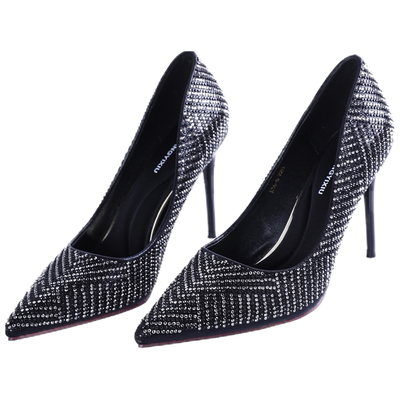
\includegraphics[width=1.45cm]{pog/hidden_16088.png}};
\node[lbl,below=1pt of r11,text=cS] {\#11: 44.1, the hidden item};
\draw[arr] (score.south) -- (r11.north);
\node[small,align=left,anchor=west] at (10.6,-2.3) {The top items are shoes too: they fit the bag and\\earrings as well, and were bundled with these\\seeds more often. Items in a seed's category\\(bags, earrings) fall below rank 6{,}000.};

\end{tikzpicture}
\end{document}
